\documentclass[9pt]{article}

\usepackage[margin=2cm]{geometry}
\usepackage{hyperref}
\usepackage{algorithm}
\usepackage{algpseudocode}
\usepackage{amsmath, amsthm, amssymb}
\usepackage{multicol}
\usepackage{tikz}
\usetikzlibrary{graphs}

\newtheorem{theorem}{Theorem}
\newtheorem{claim}{Claim}
\newtheorem{corollary}{Corollary}

\title{
    \textbf{CSE319: Modern Algorithm Design} \\
    \textbf{\large{Homework 1 Solutions}}
}
\author{
    \textbf{Submitted By:} \href{mailto:divyajeet21529@iiitd.ac.in}{Divyajeet Singh (2021529)}
    \hfill
    \textbf{Discussion Partner:} \href{mailto:siddhant21565@iiitd.ac.in}{Siddhant Rai Viksit (2021565)}
}
\date{}

\begin{document}
\maketitle

\section*{Solution 1.}
\subsection*{Part (a)}
We are given two weight functions $w_{1}$ and $w_{2}$ such that
\begin{equation}
    \label{eq:weights}
    w_{1}(e) \leq w_{1}(e') \iff w_{2}(e) \leq w_{2}(e') \quad \forall \ e, e' \in E
\end{equation}
Since the given implication \ref{eq:weights} is birectional, we can prove for any one
direction and it will hold for the other direction without loss of generality.
\begin{claim}
    \label{claim:weights-MST}
    Any MST of a graph $G = (V, E)$ with weight function $w_{1}$ is also an MST of $G$ with
    weight function $w_{2}$.
\end{claim}
\begin{quote}
\textit{Proof.}
Let $T_{1}$ be an MST of $G$ w.r.t $w_{1}$. Assume for the sake of contradiction that $T_{1}$
is not an MST of $G$ w.r.t $w_{2}$. Let $T_{2} \neq T_{1}$ be an MST of $G$ w.r.t $w_{2}$.
Then, there exists an edge $e_{2} \in T_{2} \setminus T_{1}$ such that
\begin{equation}
    \label{eq:weights-w2}
    w_{2}(e_{2}) < w_{2}(e_{1}) \implies w_{1}(e_{2}) < w_{1}(e_{1}) \quad (\text{By }\ref{eq:weights})
\end{equation}
for some edge $e_{1} \in T_{1} \setminus T_{2}$. Adding $e_{2}$ to $T_{1}$ creates a cycle
in $T_{1}$ containing both $e_{1}$ and $e_{2}$. Then, $T^{*} = T_{1} \setminus \{e_{1}\} \cup \{e_{2}\}$ is a spanning tree with
weight
\begin{equation}
    \label{eq:weights-Tstar}
    w_{1}(T^{*}) = w_{1}(T_{1}) - w_{1}(e_{1}) + w_{1}(e_{2}) < w_{1}(T_{1})
\end{equation}
which contradicts the assumption that $T_{1}$ is an MST w.r.t. $w_{1}$.
\hfill $\square$
\end{quote}

\begin{corollary}
    Any MST of a graph $G = (V, E)$ with weight function $w_{2}$ is also an MST of $G$ with
    weight function $w_{1}$.
\end{corollary}
\begin{quote}
\textit{Proof.}
    Without loss of generality in \ref{eq:weights} and by Claim \ref{claim:weights-MST},
    the corollary holds by swapping $w_{1}$ and $w_{2}$.
\hfill $\square$
\end{quote}

\subsection*{Part (b)}
We need to show that any MST of a graph $G$ has the weight $n - W + \sum_{i=1}^{W-1} \kappa_{i}$,
where $\kappa_{i}$ is the number of components in the subgraph $G_{i}$ of $G$ having edges of weight
at most $i$, and the edge weights are integers in the range $\{ 1, 2, \dots, W \}$.
\begin{claim}
    \label{claim:kappa-sequence}
    The sequence $\kappa_{0}, \kappa_{1}, \dots, \kappa_{W-1}, \kappa_{W}$ is monotonically
    non-increasing.
\end{claim}
\begin{quote}
\textit{Proof.}
We use $\kappa_{0}$ to denote the subgraph $G_{0}$ of $G$ with edges having weight at most $0$,
i.e. no edges. This means $G_{0}$ has no edges, i.e. $G_{0}$ has $n$ components. Then,
$\kappa_{0} = n$. If $W$ is the weight the heaviest edge in $G$, then $G_{W}$ contains all
edges of $G$, i.e. $G_{W}$ has only and exactly $1$ component. \\
Suppose there is no edge in the graph with weight $w \in \{ 1, 2, \dots, W \}$. Then, $G_{w}$
contains no extra edges as compared to $G_{w-1}$, i.e. $\kappa_{w-1} = \kappa_{w}$. \\
Finally, in the general case for any $G_{i}$ and $G_{i+1}$ having $\kappa_{i}$ and
$\kappa_{i+1}$ components respectively, we have $\kappa_{i} \geq \kappa_{i+1}$, because some
edge of weight $i+1$ may or may not connect some components in $G_{i}$. If all edges of weight
$i+1$ are inside the components already present in $G_{i}$, then $\kappa_{i+1} = \kappa_{i}$.
Otherwise, they will connect some components, making $\kappa_{i+1} < \kappa_{i}$.
\hfill $\square$
\end{quote}
\begin{claim}
    \label{claim:weight-MST}
    The weight of any MST of $G$ is exactly $\sum_{i+1=1}^{W} (i + 1) (\kappa_{i} - \kappa_{i+1})$.
\end{claim}
\begin{quote}
\textit{Proof.}
We can prove the claim by showing that any correct MST-producing algorithm, say Kruskal's, produces
an MST with the given weight. This is simple to see. In the sorted order of edges on the $i^{th}$
iteration, the algorithm considers all edges of weight at most $i$ if all edge weights are in the
range $\{ 1, 2, \dots, W \}$. $\kappa_{i} - \kappa_{i+1}$ represents the number of edges that are
required to connect the components in $G_{i}$ to form $G_{i+1}$. The weight of these edges is
exactly $i+1$. So, Kruskal's algorithm adds $\kappa_{i} - \kappa_{i+1}$ many edges of weight $i+1$
to make the MST for every weight $i$.
Since Kruskal's algorithm always produces a correct MST, the weight of any MST of $G$ is exactly
the given expression.
\hfill $\square$
\end{quote}
\begin{claim}
    The weight of any MST of $G$ is exactly $n - W + \sum_{i=1}^{W-1} \kappa_{i}$.
\end{claim}
\begin{quote}
\textit{Proof.}
We show that the expression in Claim \ref{claim:weight-MST} is equal to the given expression.
\begin{align}
    \begin{split}
        \sum_{i+1=1}^{W} (i + 1) (\kappa_{i} - \kappa_{i+1})
        &= \sum_{i=0}^{W-1} (i + 1) (\kappa_{i} - \kappa_{i+1}) \\
        &= \sum_{i=0}^{W-1} i \kappa_{i} + \sum_{i=0}^{W-1} \kappa_{i} - \sum_{i=0}^{W-1} (i + 1) \kappa_{i+1} \\
        &= \sum_{i=0}^{W-1} i \kappa_{i} + \sum_{i=0}^{W-1} \kappa_{i} - \sum_{i=1}^{W} i \kappa_{i} \\
        &= n - W + \sum_{i=1}^{W-1} i \kappa_{i} + \sum_{i=1}^{W-1} \kappa_{i} - \sum_{i=1}^{W-1} i \kappa_{i} \\
        &= n - W + \sum_{i=1}^{W-1} \kappa_{i}
    \end{split}
\end{align}
where we crucially use the fact that $\kappa_{0} = n$ and $\kappa_{W} = 1$.
\hfill $\square$
\end{quote}

\subsection*{Part (c)}
Given all edge weights in a graph $G = (V, E)$ are distinct. For the sake of contraction,
let us assume that there are two MSTs $T_{1}$ and $T_{2}$ of $G$ such that $T_{1} \neq T_{2}$.
Let $e_{1} \in T_{1} \setminus T_{2}$ be the lightest edge in $T_{1}$ that is not in $T_{2}$.
Adding $e_{1}$ to $T_{2}$ creates a cycle $C$ in $T_{2}$, since $T_{2}$ is a spanning tree.
Consider an edge $e_{2} \in C \setminus T_{1}$. Such an edge must exist, since $T_{2}$ is a
spanning tree and $e_{1}$ is not in $T_{2}$. Since $e_{2} \notin T_{1}$, then
$w(e_{1}) < w(e_{2})$, as $e_{1}$ must have been chosen, even when competing with $e_{2}$.
Then, the tree $T^{*} = T_{2} \setminus \{e_{2}\} \cup \{e_{1}\}$ is a spanning tree of $G$ having
\begin{equation}
    \label{eq:weight-T}
    w(T^{*}) = w(T_{2}) - w(e_{2}) + w(e_{1}) < w(T_{2})
\end{equation}
which contradicts the assumption that $T_{2}$ is an MST of $G$.
\hfill $\square$

\section*{Solution 2.}
\subsection*{Part (a)}
We show an implementation of the graph contraction algorithm in $O(m)$ time
in Algorithm \ref{alg:graph-contraction}.
\begin{algorithm}
    \caption{The \textsc{Contract} subroutine in $O(m)$ time.}
    \label{alg:graph-contraction}
    \begin{algorithmic}[1]
        \Procedure{Contract}{$G = (V, E)$}:
            \State \textsc{Ufds} $\gets [v_{1}, v_{2}, \dots, v_{n}]$ \Comment{A union-find data structure for all vertices $v \in V$}
            \For{$(u, v) \in E$}
                \If{$(u, v)$ is \textsc{Blue}}
                    \State \Call{Ufds-union}{$u, v$}
                \EndIf
            \EndFor
            \State $V' \gets \{ \Call{Ufds-find}{v} \mid v \in V \}$
            \State $E' \gets \{ (\Call{Ufds-find}{u}, \Call{Ufds-find}{v}): \infty \mid (u, v) \in E \}$ \Comment{A mapping of new edges to weights}
            \For{$(u, v) \in E$}
                \State $r_{u} \gets \Call{Ufds-find}{u}$
                \State $r_{v} \gets \Call{Ufds-find}{v}$
                \If{$r_{u} \neq r_{v}$}
                    \State $E'[r_{u}, r_{v}] \gets \min\{ E[u, v], E'[r_{u}, r_{v}] \}$ \Comment{Assuming a mapping of the form $E[u, v] = w_{uv}$}
                \EndIf
            \EndFor
            \State \Return $G' = (V', E')$
        \EndProcedure
    \end{algorithmic}
\end{algorithm}
\vspace*{0pt} \\
In the given implementation, we use a union-find data structure to keep track of the connected
components of the graph. The union-find disjoint set is one such data structure, using which, we
can find the root/parent of each connected component in near constant time. \\
The bottleneck of the algorithm are the loops over the edge-set $E$ of the graph. We first loop
over $E$ to identify all connected components, which is done in $O(m)$ time (since each step takes
roughly $O(1)$ time). The new vertex set $V'$ is constructed in $O(n)$ time (we can construct $V'$ by
going over $E$ as well). The new edge set $E'$ is initialized with infinite weights, and then
updated to the minimum edge weight between each pair of connected components, which is done in
$O(m)$ time. \\
So, the overall time complexity\footnote{The actual time complexity of the algorithm is $O(m + n)$,
since we incur $O(n)$ work to create the new vertex set. But I believe we assume for all practical
purposes $n \leq m$. This additional work can be avoided while using the subroutine in Boruvka's
algorithm if we contract on the fly, since we can obtain the new vertex set by finding the roots of
vertices from the edges.} of the \textsc{Contract} subroutine is $O(m)$.

\subsection*{Part (b)}
The solution to this problem requires showing a \textit{bad example} for Boruvka's algorithm,
where the number of edges in $G$ remains $\Omega(m)$ for $\Omega(\log{n})$ rounds. Consider a
line graph of $n$ vertices, having $m = n - 1$ edges.
\begin{figure}[htbp]
    \centering
    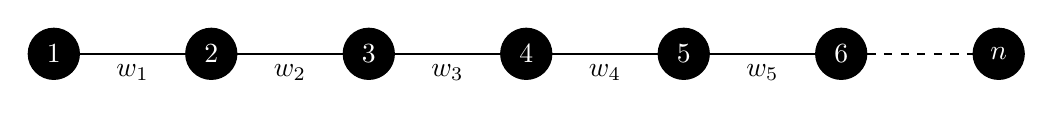
\begin{tikzpicture}
        \tikzstyle{node} = [draw, circle, minimum size=0.65cm, fill=black, text=white]
        \tikzstyle{edge} = [-, thick]
        \tikzstyle{dots} = [dashed, thick]
        \node[node] (node1) at (0,0) {$1$};
        \node[node] (node2) at (2,0) {$2$};
        \node[node] (node3) at (4,0) {$3$};
        \node[node] (node4) at (6,0) {$4$};
        \node[node] (node5) at (8,0) {$5$};
        \node[node] (node6) at (10,0) {$6$};
        \node[node] (node7) at (12,0) {$n$};
        \draw[edge] (node1) -- (node2) node[midway, below] {$w_{1}$};
        \draw[edge] (node2) -- (node3) node[midway, below] {$w_{2}$};
        \draw[edge] (node3) -- (node4) node[midway, below] {$w_{3}$};
        \draw[edge] (node4) -- (node5) node[midway, below] {$w_{4}$};
        \draw[edge] (node5) -- (node6) node[midway, below] {$w_{5}$};
        \draw[dots] (node6) -- (node7);
    \end{tikzpicture}
    \caption{A line graph with $n$ vertices with $m = n-1$ weighted edges.}
\end{figure}
\vspace*{0pt} \\
We set the weights of the edges such that
\begin{equation}
    \label{eq:weights-line}
    w_{i} = \begin{cases}
        1 & \text{if } i \in \{ 2k + 1 \mid k = 0, 1, 2, \dots \} \\
        2 & \text{if } i \in \{ 4k + 2 \mid k = 0, 1, 2, \dots \} \\
        4 & \text{if } i \in \{ 8k + 4 \mid k = 0, 1, 2, \dots \} \\
        \vdots & \vdots \\
        2^{j} & \text{if } i \in \{ 2^{j} \cdot (2k + 1) \mid k = 0, 1, 2, \dots \}
    \end{cases}
\end{equation}
In essence, we start with an unweighted graph. Weights are assigned to the edges in a
fashion similar to the Sieve of Eratosthenes. We assign weight $2^{j}$ to alternate
unweighted edges in the $j$-th round until all edges are marked. Now, we model the
behavior of Boruvka's algorithm on the above graph. \\
In the first round, each vertex has exactly one edge weighted $1$ incident on it. The
other edge incident on the vertex will be heavier, since only alternate edges have
weight $1$. These are the $\frac{m}{2}$ edges which are contracted in the first round.
We enter the second round with $\frac{m}{2} = \Omega(m)$ edges (and $\frac{n}{2}$
vertices). In the second round, each contracted vertex has exactly one edge weighted
$2$ incident on it. The other edge incident on the vertex will be heavier, since only
alternate of alternate edges have weight $2$. These edges will be contracted in the
second round. \\
It is easy to see that in general, the number of edges in the graph in the $k$-th
round will be $\frac{m}{2^{k}} = \Omega(m)$. Clearly, there will be exactly
$\log_{2}{n} = \Omega(\log{n})$ rounds of the algorithm, since the number of
vertices is halved in each round.

\subsection*{Part (c)}
We propose an $O(m \log{\log{n}})$ time algorithm to find the MST of a graph. The algorithm
is a hybrid of Boruvka's and Prim/Jarnik's algorithms. The algorithm is described in
Algorithm \ref{alg:hybrid-mst}.
\begin{algorithm}
    \caption{An $O(m \log{\log{n}})$-time algorithm to find the MST of a graph.}
    \label{alg:hybrid-mst}
    \begin{algorithmic}[1]
        \Procedure{Minimum-spanning-tree}{$G = (V, E)$}:
            \For{$i \gets 1$ to $\log{\log{n}}$}
                \State $G \gets \Call{Boruvka-round}{G}$ \Comment{Color the lightest edge of each vertex and contract the graph}
            \EndFor
            \State $T \gets \Call{Prim-Jarnik}{G}$
            \State \Return $T$
        \EndProcedure
    \end{algorithmic}
\end{algorithm}
\vspace*{0pt} \\
Let us analyze the time complexity of the algorithm. We crucially use the following facts
\begin{enumerate}
    \item Each step of the Boruvka's algorithm takes $O(m)$ time.
    \item Boruvka's algorithm halves the number of vertices in each round. So, the number
    of vertices after $k$ rounds on a graph $G$ is $\frac{n}{2^{k}}$.
    \item Prim/Jarnik's algorithm takes $O(m + n \log{n})$ time to find the MST of a graph
    when implemented using Fibonacci heaps.
\end{enumerate}
By fact 1, the $\log{\log{n}}$ rounds of Boruvka's algorithm take $O(m \log{\log{n}})$ time.
By this time, the contracted graph can contain at most
\begin{equation}
    \label{eq:vertices-contracted}
    \frac{n}{2^{\log{\log{n}}}} = \frac{n}{\log{n}} \qquad \text{(By fact 2)}
\end{equation}
vertices. For simplicity, we say that the contracted graph can still contain at most $m$ edges.
Then, the final application of Prim/Jarnik's algorithm takes (by fact 3)
\begin{equation}
    \label{eq:prim-jarnik-time}
    O\left( m + \frac{n}{\log{n}} \log{\frac{n}{\log{n}}} \right)
    = O\left(m + \frac{n}{\log{n}} \log{n} - \frac{n}{\log{n}} \log{\log{n}}\right)
    = O(m + n)
\end{equation}
time. The dominating factor thus, is the time taken by the steps of the Boruvka's algorithm.
Formally,
\begin{equation}
    \label{eq:time-complexity}
    O(m \log{\log{n}} + m + n) = O(m \log{\log{n}})
\end{equation}
Thus, the overall time complexity of the proposed Algorithm \ref{alg:hybrid-mst} is
$O(m \log{\log{n}})$.

\section*{Solution 3.}
\subsection*{Part (a)}
Algorithm \ref{alg:boruvka} describes the usual Boruvka's algorithm to find the MST of a graph.
\begin{algorithm}
    \caption{Boruvka's algorithm to find the MST of a graph.}
    \label{alg:boruvka}
    \begin{algorithmic}[1]
        \Procedure{Boruvka}{$G = (V, E)$}:
            \State $T \gets \emptyset$
            \State $\textsc{Ufds} \gets [v_{1}, v_{2}, \dots, v_{n}]$ \Comment{A union-find data structure for all vertices $v \in V$}
            \While{$|T| < n-1$}
                \For{$v_{i} \in V$}
                    \State $v_{j} \gets \arg\min_{v : (v_{i}, v) \in E} \ \{ w(v_{i}, v) \mid \Call{Ufds-find}{v_{i}} \neq \Call{Ufds-find}{v} \}$
                    \State $T \gets T \cup \{(v_{i}, v_{j})\}$
                    \State \Call{Ufds-union}{$v_{i}, v_{j}$}
                \EndFor
            \EndWhile
            \State \Return $T$
        \EndProcedure
    \end{algorithmic}
\end{algorithm}
\vspace*{0pt} \\
Since the number of vertices gets halved in each round of Boruvka's algorithm, the algorithm
requires $O(\log{n})$ rounds to find the MST of a graph with $n$ vertices. Note the following
\begin{enumerate}
    \item In each round, the algorithm takes, in total, $O(m + n)$ to identify the lightest
    edge incident on each vertex. This is because for each vertex, we might need to scan all its
    adjacent edges to find the lightest one.
    \item When implemented smartly, we can contract the graph on the fly. The union-find disjoint
    set data structure can be used to keep track of the connected components of the graph in near
    constant time. Its initialization takes $O(n)$ time.
\end{enumerate}
So, the time complexity of the Boruvka's algorithm is $O((m + n) \log{n}) = O(m \log{n})$.
Now, we are given that the edges adjacent to each vertex are stored in increasing order of
weights. This fact helps us in the following ways
\begin{enumerate}
    \item The lightest edge incident on each vertex can be identified in $O(1)$ time. For each
    vertex, this edge is the leftmost edge in its adjacency list not considered so far. This can be
    simply achieved through pointers for each vertex.
    \item The initialization of the union-find data structure still takes the initial $O(n)$ time and
    each of the union and find operations take near constant time. Thus, we have reduced the total
    time to identify the lightest edge incident on each vertex to $O(n)$.
    \item The algorithm will see each edge only and exactly once (as opposed to
    going over them multiple times to find the minimum). This scanning of each of the $m$ edges adds
    another $O(m)$ time to the algorithm.
\end{enumerate}
Thus, we have seen that we require $O(n)$ time for each of the $\log{n}$ rounds of the Boruvka's
algorithm required to find the MST, with an additional overhead of $O(m)$ to scan all the edges. So,
if the adjacency list is sorted in increasing order of weights, the time complexity of the Boruvka's
algorithm is $O(m + n \log{n})$.

\subsection*{Part (b)}
Given a list of $N$ numbers and a parameter $k$, we want to partition the list into $k$ buckets
of size at most $\left\lceil \frac{N}{k} \right\rceil$ such that each bucket contains elements
smaller than the elements in the bucket to its right. The algorithm is described in Algorithm
\ref{alg:k-partition}.
\begin{algorithm}
    \caption{An $O(N \log{k})$ algorithm to partition a list into $k$ buckets.}
    \label{alg:k-partition}
    \begin{algorithmic}[1]
        \Procedure{$k$-partial-sort}{$A[1:N]$, $k$}:
            \State $\textsc{Pivots} \gets \left\{ \frac{cN}{k} \mid c = 1, 2, \dots, k-1 \right\}$
            \For{$i \gets 1$ to $\log{k}$}
                \For{$j \gets 0$ to $2^{i}-1$}
                    \State $p \gets \left\lceil \frac{k}{2^{i}} \right\rceil$
                    \State $l \gets \textsc{Pivots} \left[ j \cdot p \right]$
                    \State $r \gets \textsc{Pivots} \left[ \min\left\{ (j+1) \cdot p, N \right\} \right]$
                    \State $m_{j} \gets \Call{Quickselect}{A[l:r], p}$
                    \State $\Call{Partition}{A[l:r], m_{j}}$
                \EndFor
            \EndFor
        \EndProcedure
    \end{algorithmic}
\end{algorithm}
\vspace*{0pt} \\
Before analysing the running time of the proposed algorithm, we make the following points.
\begin{enumerate}
    \item The algorithm modifies the input list in-place, resulting in a $k$-partially
    sorted array. We can instead choose to return the set of the final $k-1$ pivots, or return
    the groups $g_{1}$, $g_{2}$, $\dots$, $g_{k}$ as a nested list.
    \item We use two standard subroutines in the algorithm.
    \begin{enumerate}
        \item The \textsc{Quickselect} subroutine finds the $K^{th}$ smallest element of a
        list of $n$ numbers in $O(n)$ time. We use the quickselect algorithm on portions/sub-sections
        of the original array.
        \item The \textsc{Partition} subroutine partitions the list around a pivot, such
        that all elements smaller than the pivot are on the left, and all elements greater
        than (or equal to) the pivot are on the right. This can be done in $O(n)$ time for
        a list of $n$ elements.
    \end{enumerate}
\end{enumerate}
Here is an informal description of the algorithm. We identify $k-1$ evenly spaced pivot
indices in the list\footnote{These are the first $k-1$ multiples of $\left\lceil \frac{N}{k} \right\rceil$}.
We first identify the element that should sit at the $\left\lceil \frac{N}{2} \right\rceil$ position
in the sorted list and partition the list around it. Then, we repeat the same procedure for
the two halves formed after the partition - identify the element that should be at the
$\left\lceil \frac{N}{4} \right\rceil^{th}$ position in the first half, and in the second half (separately).
We then repeat this procedure for $\log{k}$ rounds\footnote{In the final iteration, $p$ becomes 1, so
we partition the sub-array of size $\left\lceil \frac{2N}{k} \right\rceil$ around each pivot}.
\begin{claim}
    \label{claim:k-partition-size}
    In the $i^{th}$ iteration, the size of each group is at most $\left\lceil \frac{N}{2^{i}} \right\rceil$.
\end{claim}
\begin{quote}
\textit{Proof.}
    The size of each group in the \textit{active area} in the list is roughly halved in each iteration. This is because
    the pivots are evenly spaced throughout the array. In each iteration, we select the central pivot of the
    current sub-array. In fact, if the size of the array is a power of $2$, the  array will be halved exactly in each iteration.
    In the $i^{th}$ iteration, the size of each group, thus, becomes at most $\left\lceil \frac{N}{2^{i}} \right\rceil$.
\hfill $\square$
\end{quote}
\begin{claim}
    \label{claim:k-partition}
    In the $i^{th}$ iteration, we get a $2^{i}$-partially sorted array.
\end{claim}
\begin{quote}
\textit{Proof.}
We can prove the claim using induction on $i$. The base case is $i = 1$, where we want to divide
the array into $2$ groups. We partition around the element which should sit in the middle of the
sorted array (i.e. its median). Clearly, the size of the 2 groups is at most $\left\lceil \frac{N}{2} \right\rceil$,
and by the partitioning property, the elements of the first group are smaller than those of the second. \\
Assume that the claim holds for some $i = I$. We prove the claim for $i = I+1$. We partitioned
the array into $2^{I}$ groups in the $I^{th}$ iteration. In the $(I+1)^{th}$ iteration, we partition
each of these $2^{I}$ groups into $2$. We partition each bucket on the pivot location in its middle.
Partitioning property guarantees the left-right sorted nature of the sub-buckets. This, in-turn, means
that finally, the elements of any group are smaller than the elements of the groups to its right.
Moreover, since the size of each group in the $I^{th}$ iteration was at most
$\left\lceil \frac{N}{2^{I}} \right\rceil$, the size of each group in the $(I+1)^{th}$ iteration
is at most $\left\lceil \frac{N}{2^{I}} \cdot \frac{1}{2} \right\rceil = \left\lceil \frac{N}{2^{I+1}} \right\rceil$
by Claim \ref{claim:k-partition-size}.
Thus, the claim holds for $i = I+1$.
\hfill $\square$
\end{quote}
\begin{corollary}
    The algorithm paritions the list into a $k$-partially sorted array.
\end{corollary}
\begin{quote}
\textit{Proof.}
    In the $(\log{k})^{th}$ iteration, the algorithm partitions the list into $k$ groups.
    By claim \ref{claim:k-partition}, the output list is $k$-partially sorted.
\hfill $\square$
\end{quote}
The time complexity of Algorithm \ref{alg:k-partition} is $O(N \log{k})$. It is clear that the outer
loop runs for $\log{k}$ iterations. Thus, we only need to show that the inner loop runs in $O(N)$
time for each $i$. Let $T(n)$ denote the time taken by the inner loop for a list of size $n$. It is
clear that the time taken is proportional to the size of the list. Then,
\begin{equation}
    T(n) = cn \quad (c > 0), \quad \text{i.e. } T(n) = O(n)
\end{equation}
In the $i^{th}$ iteration, the inner loop runs for $2^{i}$ iterations on lists of size at most
$\left\lceil \frac{N}{2^{i}} \right\rceil$. So, the total work done in the $i^{th}$ iteration is
\begin{equation}
    2^{i} \cdot T\left(\frac{N}{2^{i}}\right) = 2^{i} \cdot \frac{cN}{2^{i}} = cN = T(N) = O(N)
\end{equation}
Since we have $\log{k}$ iterations, the total time complexity of the algorithm is $O(N \log{k})$.

\subsection*{Part (c)}
If the edges adjacent to each vertex are only $k$-partially sorted, then we can achieve the following runtime.
\begin{enumerate}
    \item The time taken to find the lightest edge incident on each vertex is $O\left( \frac{m}{k} \right)$,
    since we only always need to scan the first $\frac{m}{k}$ edges of each vertex to identify the lightest edge
    \footnote{It is obvious that if you delete the first element from any $k$-partially sorted array, the resulting
    array is still $k$-partially sorted. This is because this \textit{pop} operation essentailly reduces the size of
    the first sorted bucket by 1. After multiple deletions, it will still be sufficient to scan the first $\frac{m}{k}$
    elements to find the current required minimum.}.
    We incur an extra $O(m)$ effort once, in total, by scanning all edges of the graph.
    \item We need to do this operation for each of the $n$ vertices for each of the $\log{n}$ rounds.
\end{enumerate}
This makes the final runtime of the algorithm $O\left( m + n\log{n} + \frac{m}{k}\log{n} \right)$.

\subsection*{Part (d)}
Now we design another $O(m \log{\log{n}})$-time algorithm to find the MST of a graph. The algorithm
is described in Algorithm \ref{alg:hybrid-mst-2}.
\begin{algorithm}
    \caption{An $O(m \log{\log{n}})$-time algorithm to find the MST of a graph.}
    \label{alg:hybrid-mst-2}
    \begin{algorithmic}[1]
        \Procedure{Minimum-spanning-tree}{$G = (V, E)$}:
            \For{$i \gets 1$ to $\log{\log{n}}$}
                \State $G \gets \Call{Boruvka-round}{G}$
            \EndFor
            \For{$v \in V$}
                \State $G[v] \gets \Call{$k$-partial-sort}{G[v], \log{|V|}}$ \Comment{($\log{n}$)-partially sort the edges adjacent to each vertex}
            \EndFor
            \State $T \gets \Call{Boruvka}{G}$
            \State \Return $T$
        \EndProcedure
    \end{algorithmic}
\end{algorithm}
\vspace*{0pt} \\
This algorithm is very similar to Algorithm \ref{alg:hybrid-mst} in \textbf{Problem 2 Part (c)}. We
first run $\log{\log{n}}$ rounds of Boruvka's algorithm. Then, we partially sort the edges adjacent
to each vertex to a degree of $k = \log{n}$. Finally, we run Boruvka's algorithm on the partially
sorted graph. Combined with partial sorting, this run of Boruvka's algorithm behaves like a blackbox
for any $O(m + n \log{n})$-time MST algorithm. \\
Let us analyse the full time complexity of the algorithm.
\begin{enumerate}
    \item As analysed earlier, the time taken to run $\log{\log{n}}$ rounds of Boruvka's algorithm is
    $O(m \log{\log{n}})$.
    \item After these rounds, if $m_{v}$ edges are incident on each vertex $v$, then the time taken for
    partially sorting them is $O(m_{v} \log{k})$. The total time taken to partially sort the edges adjacent
    to all vertices is thus
    \begin{equation}
        \label{eq:partial-sort-time}
        O\left( \sum_{v \in V} m_{v} \log{k} \right) = O(m \log{\log{n}}) \quad \text{Since} \sum_{v \in V} m_{v} \leq m
    \end{equation}
    \item At this stage, the graph has at most $\frac{n}{\log{n}}$ vertices and $m$ edges, as proved
    in \textbf{Problem 2 Part (c)}. It is also $(\log{n})$-partially sorted. From \textbf{Problem 3 Part (c)},
    Boruvka's algorithm runs in $O(m + n \log{n})$ time on a $(\log{n})$-partially sorted graph. So,
    the time taken to run Boruvka's algorithm on the partially sorted graph
    \begin{equation}
        O\left( m + \frac{n}{\log{n}} \log{\frac{n}{\log{n}}} \right) = O(m + n)
    \end{equation}
\end{enumerate}
So, the overall time complexity of this MST-finding algorithm is $O(m \log{\log{n}})$.

\section*{Solution 4.}
\subsection*{Part (a)}
Consider the following graph with 7 vertices and 7 edges.
\begin{figure}[htbp]
    \centering
    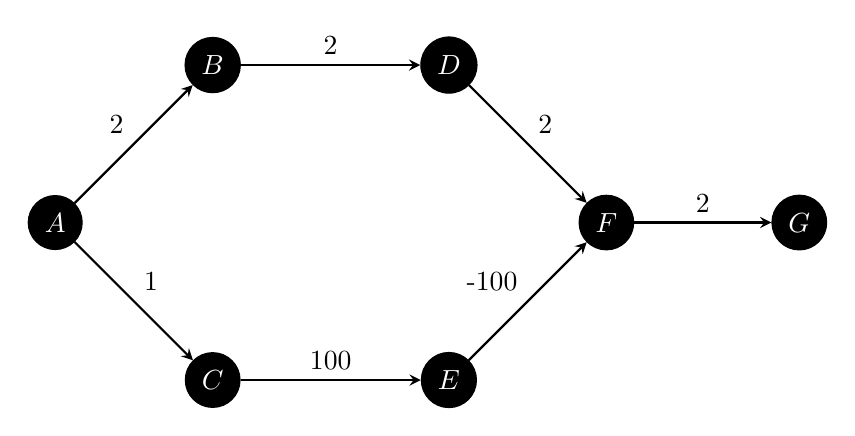
\begin{tikzpicture}[node distance=2cm, auto]
        \tikzstyle{node} = [draw, circle, minimum size=0.65cm, fill=black, text=white]
        \tikzstyle{pointer} = [-{stealth}, thick]
        \node[node] (A) at (-2,0) {$A$};
        \node[node] (B) at (0,2) {$B$};
        \node[node] (C) at (0,-2) {$C$};
        \node[node] (D) at (3,2) {$D$};
        \node[node] (E) at (3,-2) {$E$};
        \node[node] (F) at (5,0) {$F$};
        \node[node] (G) at (7.45,0) {$G$};
        \path[pointer]
        (A) edge node {2} (B)
        (A) edge node {1} (C)
        (B) edge node {2} (D)
        (C) edge node {100} (E)
        (D) edge node {2} (F)
        (E) edge node {-100} (F)
        (F) edge node {2} (G);
    \end{tikzpicture}
    \caption{A graph with 1 negative weight edge.}
\end{figure}
\vspace*{0pt} \\
Table \ref{tab:dijkstra} lists the steps of Dijkstra's algorithm for the above graph.
\begin{table}[htbp]
    \centering
    \begin{tabular}{c|c|cccccccc}
        \textsc{Iteration} & \textsc{Node} & $A$ & $B$ & $C$ & $D$ & $E$ & $F$ & $G$ \\ \hline
        0 & & 0 & $\infty$ & $\infty$ & $\infty$ & $\infty$ & $\infty$ & $\infty$ \\
        1 & $A$ & 0 & 2 & 1 & $\infty$ & $\infty$ & $\infty$ & $\infty$ \\
        2 & $C$ & 0 & 2 & 1 & $\infty$ & 100 & $\infty$ & $\infty$ \\
        3 & $B$ & 0 & 2 & 1 & 4 & 100 & $\infty$ & $\infty$ \\
        4 & $D$ & 0 & 2 & 1 & 4 & 100 & 6 & $\infty$ \\
        5 & $F$ & 0 & 2 & 1 & 4 & 100 & 6 & 8 \\
        6 & $G$ & 0 & 2 & 1 & 4 & 100 & 6 & 8 \\
        7 & $E$ & 0 & 2 & 1 & 4 & 100 & 1 & 8
    \end{tabular}
    \caption{Table showing the computed \textit{shortest} distances at each step.}
    \label{tab:dijkstra}
\end{table}
It is easy to see that the shortest distance from $A$ to $G$ is 3, but Dijkstra's algorithm
computes it as 8.

\subsection*{Part (b)}
We prove the given claim (slightly modified to ease of understanding).
\begin{claim}
    If a node $v$ is such that the shortest path from the source $s$ to $v$ contains
    at most $K$ negative-length edges, then running Dijkstra's algorithm $K+1$ times
    computes the length of this shortest $s$-$v$ path.
\end{claim}
\begin{quote}
\textit{Proof.}
The claim can be proven using induction on $K$. The base case, $K = 0$, is trivially true,
since if the shortest $s$-$v$ path has no negative-length edges, then Dijkstra's algorithm
computes the correct shortest path length in $1$ iteration. \\
We assume that the claim holds true for some $K = k$, and prove the claim for $K = k+1$. \\
Let the shortest path between $s$ and $v$ be $P_{sv} = s \rightarrow v_{1:n} \rightarrow v =
s \rightarrow v_{1} \rightarrow v_{2} \rightarrow \dots \rightarrow v_{n} \rightarrow v$. Let $P_{sv}$ contain $k+1$ negative edges.
Let us say the $(k+1)^{th}$ negative edge is between $v_{i}$ and $v_{i+1}$. By induction hypothesis,
the $(k+1)^{th}$ iteration produces the correct distance for $v_{i}$. In fact, it also produces
the correct distance for $v_{i+1}$, since the algorithm would update the path-lengths of
$v_{i}$'s neighbors. Note that the labels of $v_{i+2:n}$ and $v$ may or may not be correct.
This is because if $v_{i+1}$ was already marked, then the labels of $v_{(i+2):n}$ and $v$ would
not be updated to their correct value.
Then, one additional iteration is sufficient to update the distance labels
of $v_{(i+1):n}$ and $v$, thereby computing the length of the shortest
$s$-$v$ path.
\hfill $\square$
\end{quote}

\section*{Appendix}

\subsection*{Problem 2 (b)}
The example given as a solution to this problem may not be correct. The line graph of $n$ vertices
is a painfully obvious planar graph with $n-1 \leq 3n - 6$ edges. This means that Boruvka's
algorithm runs in $O(n)$ time, which sounds reasonable, as the effort required in each round
goes down by half. As $n$ decreases, $m$ decreases along with it. However, a confusion arises when
we think that $\frac{m}{2^{k}} = \Omega(m)$.

\end{document}